% Evaluation as Infrastructure — arXiv preprint (cs.SE).
% Build:  latexmk -pdf main.tex
%
% This is the NAMED preprint version. For a double-anonymous CAIN submission,
% swap in the IEEE conference class, remove the author block, replace the
% repository URL in §8 with an anonymised artifact link, and put the
% self-citations in the third person.

\documentclass[11pt,a4paper]{article}

\usepackage[utf8]{inputenc}
\usepackage[T1]{fontenc}
\usepackage{lmodern}
\usepackage[margin=1in]{geometry}
\usepackage{booktabs}
\usepackage{tabularx}
\usepackage{longtable}
\usepackage{array}
\usepackage{microtype}
\usepackage{listings}
\usepackage{xcolor}
\usepackage{tikz}
\usetikzlibrary{arrows.meta, positioning, fit, backgrounds}
\usepackage[hidelinks]{hyperref}
\usepackage{cleveref}

\definecolor{codebg}{HTML}{F7F7F7}
\definecolor{keyc}{HTML}{0F766E}

\lstdefinestyle{json}{
  basicstyle=\ttfamily\scriptsize,
  backgroundcolor=\color{codebg},
  frame=single, rulecolor=\color{lightgray},
  breaklines=true, showstringspaces=false,
  stringstyle=\color{keyc},
  columns=fullflexible,
  xleftmargin=1em, framexleftmargin=1em,
}

\newcolumntype{L}[1]{>{\raggedright\arraybackslash}p{#1}}

\title{\textbf{Evaluation as Infrastructure:}\\
Deterministic Regression Gating for Evidence-Grounded AI Systems in Production}

\author{Nick Lamb\\
\small PharmaTools.AI\\
\small \texttt{info@pharmatools.ai}}

% Fixed rather than \today: the PDF must not silently change its own date every
% time it is rebuilt. Bump this deliberately when a new version is deposited.
\date{14 July 2026}

\begin{document}
\maketitle

\begin{abstract}
\noindent
AI systems are increasingly deployed in domains where an answer is only useful if it can be
justified from source material: clinical claim verification, patient-facing simplification of
medical text, de-identification, and retrieval over biomedical authorities. Prevailing evaluation
practice measures whether outputs are \emph{plausible}, often by using a second language model as a
judge. That approach is costly, non-deterministic, and difficult to gate a release on. We present
OpenGATE, an open-source framework that treats evaluation of evidence-grounded AI as continuous
engineering infrastructure: hand-labelled gold datasets, deterministic scorers (no LLM-as-judge),
reproducible scorecards, and a per-adapter regression gate wired into continuous integration. The
framework defines five \emph{capabilities} (evidence QA, redaction, simplification, retrieval,
and generic grounding) behind a small adapter contract, so one methodology evaluates systems of
different task shapes. We report experience applying OpenGATE to four production systems operated by
a single small organisation, including an MHRA-registered medical device. On its first run, three of
the four systems yielded real defects that human review and conventional testing had missed: a
silent parse-failure mode affecting roughly half of multi-claim verdicts, two name-capture failures
in a de-identification engine, and a simplifier that dropped an antibiotic dose from a discharge
summary. Each was fixed and re-verified by the same gate, typically the same day. The fourth system
passed cleanly, and the defect that run exposed was in the benchmark itself: a case-authoring
helper that proposed an anchor which could not fail. This illustrates a risk that applies to any gold
set, including ours: a benchmark can fail by passing. We also compare the deterministic
scorers directly against two LLM-judge faithfulness implementations (RAGAS, DeepEval) over a frozen
corpus with injected defects, and report a two-sided result: the judges detect meaning inversions
that deterministic checking cannot see (4/5 and 5/5 versus 0/5), while both judges flag one of four
clean production outputs in every one of five repeats, are near-blind to omission (0/5 and 1/5 versus
5/5), and cost roughly \$8--11 per 1{,}000 evaluations versus zero. Most consequentially, the two
judge libraries disagree about what their shared metric name means: on outputs asserting figures
absent from the source, one detects 5/6 and the other 0/6. A team adopting ``LLM-as-judge
faithfulness'' without reading the implementation is not choosing a level of rigour so much as
choosing, unknowingly, which failure mode to be blind to. OpenGATE is available under the MIT licence.
\end{abstract}

\noindent\textbf{Keywords}: AI engineering, evaluation, regression testing, retrieval-augmented
generation, grounding, hallucination, continuous integration, medical AI

\section{Introduction}

Software engineering answered the question ``how do we change code without breaking it?'' decades
ago: automated tests, run on every change, gating every release. AI-enabled systems mostly lack an
equivalent. Teams ship prompt changes, model upgrades, and pipeline refactors on the strength of
spot checks and anecdote, because the standard evaluation tools measure the wrong thing at the wrong
time: benchmark suites measure a \emph{model} before integration, and LLM-as-judge harnesses measure
\emph{plausibility} at a per-run cost and variance that make them awkward to gate a build on.

For a class of systems we call \emph{evidence-grounded}, whose core promise is that every output is
justified by identified source material, this gap is acute. The failure modes that
matter in production are quiet and specific: a supporting passage that does not exist verbatim in the
cited source; a claim reworded before verification; a patient identifier that survives
de-identification; a medication dose silently dropped from a simplified letter; an author's name lost
by a retrieval parser. None of these are visible in aggregate quality scores, and none require
semantic judgment to detect. They are checkable, deterministically, against labelled expectations.

This paper reports the design of, and production experience with, \textbf{OpenGATE} (Open Grounded AI
Testing \& Evaluation), an open-source framework built on three positions:

\begin{enumerate}
  \item \textbf{Evaluation is infrastructure, not an experiment.} Scorers run in CI; a regression
  against a committed per-adapter baseline fails the build. The unit of value is not a leaderboard
  number but a \emph{prevented deployment}.
  \item \textbf{Judgment belongs in the gold set, not in a judge model.} All scorers are
  deterministic functions of system output and hand-labelled expectations. This trades semantic
  coverage for reproducibility, zero marginal cost, named failures, and CI-compatible stability. We
  measure that trade in \Cref{sec:exp2} and criticise it in \Cref{sec:limits}.
  \item \textbf{The methodology travels; only the gold set changes.} A small adapter contract lets
  one framework evaluate systems of different task shapes. We define five capabilities: evidence QA,
  redaction, simplification, retrieval, and generic grounding for RAG.
\end{enumerate}

Our primary contribution is empirical: an experience report across four production systems
(a clinical claim verifier, a de-identification engine, a patient-language simplifier registered as a
Class I medical device, and a biomedical retrieval server), all operated by a single small
organisation. On its first run, three of the four systems yielded at least one real, previously
unknown defect (\Cref{sec:ledger}), each subsequently fixed and re-verified by the same gate,
typically within one day. The fourth passed cleanly, and the defect that run did surface was in the
benchmark itself: a case-authoring helper that proposed an anchor incapable of failing. We report it because it names the failure mode this class of work is most exposed to: a gold set
can be green and worthless.

We further contribute a controlled comparison against LLM-as-judge faithfulness metrics
(\Cref{sec:exp2}), the framework's design (capabilities, adapter contract, per-adapter baselines), a
\emph{tracked-known-gap lifecycle} that operationalises honest limitation reporting
(\Cref{sec:knowngap}), and a discussion of what deterministic scoring can and cannot see.

\section{Related Work}

\paragraph{LLM evaluation frameworks.}
General-purpose harnesses such as RAGAS~\cite{es2024ragas} and DeepEval~\cite{ip2026deepeval}
provide metric libraries for LLM applications; RAGAS in particular targets RAG faithfulness. Most
faithfulness metrics in these frameworks are LLM-as-judge: a grader model scores the output.
LLM-as-judge has documented strengths for open-ended quality~\cite{zheng2023judging,liu2023geval} and
well-documented weaknesses: position and verbosity effects and self-enhancement
bias~\cite{zheng2023judging}, unfairness under candidate reordering~\cite{wang2024unfair},
self-preference for a judge's own generations~\cite{panickssery2024selfpref}, and a spread of
cognitive biases benchmarked systematically by Koo et al.~\cite{koo2024biases}. Several of these
critiques come from the judge literature itself; G-Eval's own authors flag a bias toward
LLM-generated text~\cite{liu2023geval}.

Our contribution to this thread is empirical and, we think, underappreciated: in
\Cref{sec:exp2} we show that two widely used frameworks ship a metric under the same name,
\emph{faithfulness}, and do not mean the same thing by it, to the point of assigning scores of
$0.000$ and $1.000$ to the same fabrication. The literature on judge \emph{bias} presumes the
judges are at least measuring the same construct. Ours is a prior question: whether they are.
OpenGATE is positioned as a complement, not a replacement: it specialises in the deterministic
subset of grounding properties that can gate CI, and delegates open-ended quality to human review or
to judge-based frameworks used as a non-blocking signal.

\paragraph{Reference-based factuality checking.}
FEVER~\cite{thorne2018fever}, FActScore~\cite{min2023factscore}, SummaC~\cite{laban2022summac}, and
QAFactEval~\cite{fabbri2022qafacteval} measure factual consistency against sources, largely via
trained models over public benchmarks. OpenGATE differs in unit of deployment (a CI gate over an
organisation's own gold cases, not a benchmark) and in scoring mechanics (string- and
structure-level determinism rather than model inference).

\paragraph{Regression testing for ML systems.}
The SE4AI literature has long argued that ML components need continuous, system-level testing:
hidden technical debt accrues at the system boundary~\cite{sculley2015debt}, production readiness
needs an explicit rubric~\cite{breck2017mltest}, and industrial ML teams report testing and
evaluation as a first-order engineering problem~\cite{amershi2019se4ml}. OpenGATE can be read as an
instantiation of that argument for the specific contract of evidence-groundedness, with an empirical
ledger from production.

\section{Design Principles}

\paragraph{P1 --- Deterministic scoring.}
Every scorer is a pure function of (system output, gold case). No grader model, no sampling, no
network beyond the system under test. Consequences: scores are reproducible bit-for-bit; a failing
case names the exact expectation violated (\texttt{DROPPED FACT: anchor `500 mg' absent}); offline
scorers cost nothing and run on every commit; and the framework cannot be gamed by persuading a
judge. The cost is coverage: paraphrase-level semantic error is out of scope unless it disturbs an
anchor, number, contract, or structural invariant. We measure that floor in \Cref{sec:exp2}.

\paragraph{P2 --- Gold sets as the locus of judgment.}
Human judgment enters exactly once: when a case is labelled. Cases are versioned JSON documents with
a documented schema and labelling guide. All bundled cases are synthetic (test-range NHS numbers
valid under modulus-11, Ofcom-reserved phone numbers, fictitious people), so the gold set itself is
publishable.

\paragraph{P3 --- Capabilities behind a thin adapter.}
An adapter is one file with two required exports (\texttt{onlineAvailable},
\texttt{onlineConfigHint}) plus at least one complete capability: \texttt{qa} (claim splitting plus
verdicts against references), \texttt{redaction}, \texttt{simplify}, \texttt{retrieval}, or
\texttt{grounding}. Adapters are validated at load with fail-fast messages naming any missing export.
A configuration-driven HTTP adapter covers REST-backed systems without code.

\paragraph{P4 --- Regression gating with per-adapter baselines.}
\texttt{-{}-baseline} commits a reference scorecard per adapter; subsequent runs print per-metric
deltas and \texttt{-{}-ci} fails the build on any drop in a rate metric. Scorecards are stamped with
the git SHA and, where relevant, a \texttt{run\_model} label, so the results directory doubles as a
measured model comparison (accuracy $\times$ hallucination $\times$ latency $\times$ token cost).

\paragraph{P5 --- Known gaps are tracked, not hidden.}
Where the system under test does not yet handle a phenomenon, the gold case records it as a
\emph{known gap} rather than a failure. The scorer reports \texttt{knownGap\_open} /
\texttt{knownGap\_closed}; when an engine fix lands, the flip to \emph{closed} is itself the
verification, and the entity is promoted to gold (\Cref{sec:knowngap}).

\section{The Framework}

\subsection{Architecture}

\begin{figure}[t]
\centering
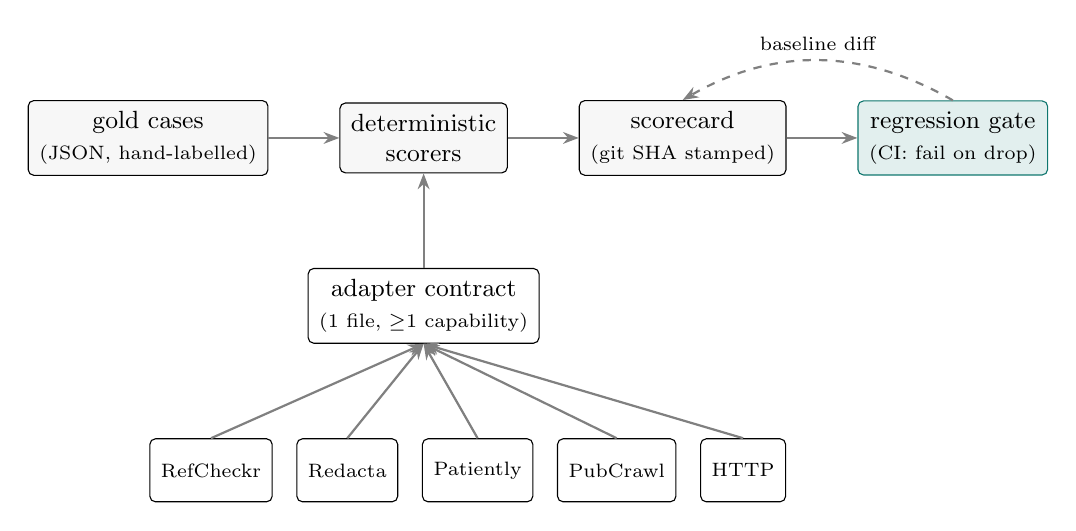
\begin{tikzpicture}[
  node distance=6mm and 9mm,
  box/.style={draw, rounded corners=2pt, align=center, minimum height=8mm, font=\small, inner sep=4pt},
  core/.style={box, fill=codebg},
  sys/.style={box, fill=white},
  gate/.style={box, fill=keyc!12, draw=keyc},
  arr/.style={-{Stealth[length=2mm]}, thick, gray}
]
\node[core] (gold) {gold cases\\\scriptsize (JSON, hand-labelled)};
\node[core, right=of gold] (scorers) {deterministic\\scorers};
\node[core, right=of scorers] (card) {scorecard\\\scriptsize (git SHA stamped)};
\node[gate, right=of card] (ci) {regression gate\\\scriptsize (CI: fail on drop)};

\node[box, below=12mm of scorers, fill=white] (adapter)
  {adapter contract\\\scriptsize (1 file, $\geq$1 capability)};

% Systems under test: one evenly spaced row, laid out left-to-right in a chain so
% the boxes cannot collide. (An earlier version positioned them with negative
% offsets relative to the narrower parent node, which overlapped them.)
\node[sys, below=12mm of adapter, xshift=-27mm] (s1) {\scriptsize RefCheckr};
\node[sys, right=3mm of s1] (s2) {\scriptsize Redacta};
\node[sys, right=3mm of s2] (s3) {\scriptsize Patiently};
\node[sys, right=3mm of s3] (s4) {\scriptsize PubCrawl};
\node[sys, right=3mm of s4] (s5) {\scriptsize HTTP};

\draw[arr] (gold) -- (scorers);
\draw[arr] (scorers) -- (card);
\draw[arr] (card) -- (ci);
\draw[arr] (adapter) -- (scorers);
\foreach \s in {s1,s2,s3,s4,s5} \draw[arr] (\s.north) -- (adapter.south);
\draw[arr, dashed] (ci.north) to[out=150,in=30]
  node[above, font=\scriptsize, black] {baseline diff} (card.north);
\end{tikzpicture}
\caption{Gold cases and deterministic scorers produce a SHA-stamped scorecard, which is diffed
against a committed per-adapter baseline; any drop in a rate metric fails the build. Systems under
test attach through a one-file adapter, so the same scorers evaluate four differently shaped
products, plus any REST-backed system, via the configuration-driven HTTP adapter, without code.}
\label{fig:arch}
\end{figure}

The runner discovers gold cases, loads and validates one adapter, executes each scorer (offline
scorers always; online scorers when \texttt{-{}-online}), prints named failures, writes a versioned
scorecard, and diffs against the adapter's baseline (\Cref{fig:arch}). A self-contained HTML report
renders pass/fail, deltas, and every named failure. The deterministic grounding core also ships as a
Python package, an MCP server (so agents can verify their own answers inline), and a Docker image:
one check, several surfaces.

\subsection{Scorers}

\begin{table}[t]
\centering
\small
\begin{tabularx}{\textwidth}{l l X}
\toprule
\textbf{Scorer} & \textbf{Capability} & \textbf{What it gates (deterministically)}\\
\midrule
citation detection & qa & citation markers parsed from prose (numeric, superscript, author--year); per-claim exact-set rate and Jaccard\\
claim extraction & qa & the claims a system splits out match gold claims; non-claims rejected (F1)\\
verdict accuracy & qa & six-class verdict against the cited reference; passage hallucination (a quoted passage absent from the source)\\
redaction & redaction & identifier recall, zero-leak check, word-level scan for partially redacted names\\
simplification & simplify & anchor recall (facts that must survive), fabricated numbers, output-length contract, readability (reported, not gated)\\
retrieval & retrieval & required fields present; anchors on parsed values (author surnames, year, abstract sections); structural invariants\\
grounding & grounding & answer-anchor recall, no ungrounded numbers, abstention when the context cannot answer\\
\bottomrule
\end{tabularx}
\caption{The seven scorers. Every one is a pure function of (system output, gold case): no grader
model, no sampling.}
\label{tab:scorers}
\end{table}

\Cref{tab:scorers} lists the scorers. Two design details matter beyond the table. First,
\textbf{word-level leak scanning} in redaction: a full-string check would miss a partially redacted
name (\texttt{[PATIENT\_1] O'Brien} removes the labelled value yet leaks the surname), so name-typed
anchors are also scanned word-by-word, with known-gap values excused. Second,
\textbf{paraphrase-tolerant faithfulness} in simplification: rewritten text is paraphrase \emph{by
design}, so prose is never compared verbatim. Instead critical facts must survive (anchors with
aliases: ``500 mg'' $\approx$ ``500mg''), every output number must trace to the source or a declared
allowance, and declared length contracts are enforced.

\subsection{What a gold case looks like}

\begin{lstlisting}[style=json, caption={A simplification gold case. The anchors are the facts whose
loss would be a safety event; \texttt{allowedNewNumbers} whitelists numbers a faithful rewrite may
introduce (here, ``3 times a day'' for ``three times daily''); the contract encodes the product's
documented Brief-mode output shape.}, label={lst:case}]
{
  "id": "simplify-discharge-brief",
  "kind": "simplification",
  "audience": "Adult", "tone": "Informative", "length": "Brief",
  "text": "Discharge summary: You were admitted with community-acquired pneumonia.
           You have been started on amoxicillin 500 mg three times daily for 5 days.
           Please see your GP in 2 weeks for review. Return to hospital if you
           develop worsening breathlessness or a fever above 38 degrees.",
  "anchors": [
    { "value": "amoxicillin" },
    { "value": "500 mg",  "aliases": ["500mg", "500 milligrams"] },
    { "value": "5 days",  "aliases": ["five days"] },
    { "value": "2 weeks", "aliases": ["two weeks"] },
    { "value": "38",      "aliases": ["38C", "38 degrees"] }
  ],
  "allowedNewNumbers": ["3"],
  "maxBullets": 3,
  "maxWordsPerBullet": 20
}
\end{lstlisting}

\subsection{The known-gap lifecycle}
\label{sec:knowngap}

Label honestly $\rightarrow$ the scorer reports the gap as open, not failing $\rightarrow$ fix the
engine $\rightarrow$ the same run flips \texttt{knownGap\_closed} $\rightarrow$ promote the entity to
gold $\rightarrow$ the gate now defends the fix forever. \Cref{sec:ledger} shows this lifecycle
executing three times in one day against a production de-identification engine. The point is
cultural as much as technical: it gives limitation reporting the same lifecycle as test-driven
development, so admitting a gap is the first step of fixing it rather than an embarrassment to be
deferred.

\section{Systems Under Test}

\begin{table}[h]
\centering
\small
\begin{tabularx}{\textwidth}{l X l l}
\toprule
\textbf{System} & \textbf{Task} & \textbf{Capability} & \textbf{Deployment context}\\
\midrule
RefCheckr & verify clinical claims against cited references & qa & commercial web app + Word add-in\\
Redacta & de-identify clinical text on device & redaction & npm/PyPI/CLI/MCP/iOS\\
Patiently AI & simplify medical text for patients & simplify & MHRA-registered Class I device\\
PubCrawl & retrieval over PubMed/ClinicalTrials.gov & retrieval & MCP server + library\\
\bottomrule
\end{tabularx}
\caption{Four production systems, one operator (PharmaTools.AI), four task shapes.}
\label{tab:systems}
\end{table}

\section{Experience: the Found-and-Fixed Ledger}
\label{sec:ledger}

\begin{table}[t]
\centering
\footnotesize
\begin{tabularx}{\textwidth}{l L{2.6cm} X l}
\toprule
\textbf{System} & \textbf{Class} & \textbf{Defect and fix} & \textbf{Verified}\\
\midrule
RefCheckr & defect (silent) &
Non-JSON model responses silently defaulted to ``Not Supported'', affecting ${\approx}50\%$ of
multi-claim verdicts. Fix: enforced structured output; parse failures $\rightarrow$ 0. &
same day\\
RefCheckr & defect (intermittent) &
Same defect class on a second endpoint (claim splitting), as an intermittent total failure, visible
only because the eval runs repeatedly. &
same day\\
RefCheckr & improvement &
Model selection across three tiers on one gold set: mid tier halved passage hallucination
(5.8\% $\rightarrow$ 2.4\%); a reasoning tier scored higher verdict accuracy (82.8\% exact) but
hallucinated passages at 15.1\%, which disqualifies it for an evidence tool. &
3 repeats\\
Redacta & defect (safety) &
Relation phrase (``Next of kin:'') consumed the region, so the inner name never matched;
apostrophe surnames (``O'Brien'') fell out of capture. Both fixed in the TS engine and its Python
port. &
\texttt{knownGap\_closed: 2}\\
Redacta & known gap closed &
Street-address lines: tracked as an open gap, then closed. Final: 100\% recall on 25 identifiers,
zero leaks. &
same week\\
Patiently AI & defect (safety) &
Anchor recall 86\%: an antibiotic dose vanished from a Brief-mode discharge summary. Root cause: the
composed prompt carried no faithfulness rule. Fix applied additively to three product-specific tone
keys (shared backend). &
100\% recall\\
Patiently AI & defect (safety) &
Later re-capture: an \emph{invented} reference range (``above 12 g/dL'') absent from the source. The
earlier rule forbade \emph{omitting} numbers and was silent on \emph{inventing} them. Fix: explicit
no-fabrication clause. &
0 fabrications\\
PubCrawl & \textbf{benchmark defect} &
System passed clean (fidelity 1.0, 8 checks). The case-authoring helper took the \emph{last} token of
``Surname ForeName Initials'' and proposed the anchor \texttt{contains:\,"J"}: a middle initial, and
a check that could not fail. Helper fixed; case rebuilt. &
8/8 checks\\
\bottomrule
\end{tabularx}
\caption{The found-and-fixed ledger. \emph{Class} separates defects from improvements, and both from
the one finding that was a defect in the evaluation tooling rather than in a system under test.}
\label{tab:ledger}
\end{table}

\paragraph{RefCheckr --- silent verdict loss.}
The first harness runs measured a parse-failure mode in batch verification: model responses that were
not strict JSON were silently defaulted to ``Not Supported'', affecting ${\approx}50\%$ of
multi-claim verdicts. A later live-production run caught the \emph{same defect class} on a second
endpoint as an intermittent total failure, visible only because the eval runs repeatedly. The
framework also drove an evidence-based model selection (\Cref{tab:ledger}), in which the incumbent
tier was replaced on measured numbers: per-1{,}000-claim cost was computed from observed token usage,
not list-price estimates.

\paragraph{Redacta --- two name-capture failures and a closed feature gap.}
On the first run against a new five-case gold set, redaction recall was 86\%. Two distinct capture
bugs were responsible, both fixed in the shared TypeScript engine and its Python port and confirmed
by the gate (\texttt{knownGap\_closed: 2}). A tracked feature gap (street-address lines) was closed
the same way days later. Final scorecard: 100\% recall on 25 identifiers, zero leaks, no open gaps.
This is the known-gap lifecycle (\Cref{sec:knowngap}) running end to end, three times, in a day.

\paragraph{Patiently AI --- dropped specifics, then invented ones.}
First production run: anchor recall 86\%. An antibiotic dose had vanished from a Brief-mode discharge
summary. Root cause: the composed prompt (audience + tone + length) contained no faithfulness rule at
all. The fix had a shared-backend constraint (the prompt map also serves a second product whose
professional audience is deliberately instructed to introduce trial figures), so the preservation rule
was added \emph{additively} to the three product-specific tone keys. Next run: 100\% anchor recall,
zero dropped facts, zero fabrications.

That result was a \emph{single run}. Capturing fresh outputs months later for the judge comparison
(\Cref{sec:exp2}), the same gold case produced a fabricated number. The simplifier volunteered a
reference range absent from the source (``\emph{Normally, we like to see a haemoglobin level above
12 g/dL}''), against a letter that never mentions 12. The figure is clinically correct; it is simply
not in the document the model was given.

The diagnosis is the interesting part. The faithfulness rule added by the earlier fix \emph{was}
reaching the relevant prompt key. It had simply been written against the failure we had already seen:
it said \emph{never omit or change the numbers}. It forbade \emph{losing} a figure and was silent on
\emph{inventing} one. A prompt hardened against the last defect was not thereby hardened against the
next, and only a check that runs on every change would notice. The fix adds an explicit
no-fabrication clause with an instruction to describe the result in words instead (``lower than
usual''), since a bare prohibition tends to produce evasions. Verification, by the same gate that
caught it: anchor recall 100\% (14/14), zero dropped facts, zero fabricated numbers, zero contract
violations. Nor was there any sign of the regression the fix might plausibly have caused, in which a
model told to be careful with numbers becomes reticent and drops them instead.

\paragraph{PubCrawl --- the system passed, and the benchmark failed.}
PubCrawl is the one system under test that produced no defect on its first run: fidelity 1.0
across 8 checks against the live production server. The defect was in the evaluation tooling. OpenGATE
ships a helper that drafts a gold case from a real fetched record, and it derived the author anchor by
taking the \emph{last} token of the author string. PubCrawl returns authors as ``Surname ForeName
Initials'', so the last token is a middle initial, and the helper proposed the anchor
\texttt{contains:\,"J"}. A gold case built on that anchor would have passed against almost any record
in PubMed: a check that cannot fail, which is worse than no check, because it reports green.

We report this as a finding \emph{against the benchmark}, because that is what it was. It is also the
sharpest illustration of a risk that applies to every gold set in this paper, our own included: a
benchmark can fail by passing. A weak anchor produces a green scorecard and a false sense of coverage, and nothing
in a deterministic scorer will tell you that the fact you pinned was not worth pinning. That is a
human judgment, which is why gold-label quality (\Cref{sec:limits}) is this framework's most exposed
assumption and not an incidental one.

\paragraph{Cross-cutting observations.}
\emph{(1) First-run yield was 3 of 4.} Three of the four systems yielded at least one real defect on
first evaluation, consistent with having been shipped under conventional review but without a
grounding-specific gate. The fourth came back clean. We note this rather than rounding it up: a claim
that \emph{every} system fails first contact is the kind of claim that sounds like advocacy.
\emph{(2) The eval-first workflow held.} In the largest change (adding author--year citation support
end to end), gold cases were written before implementation; planning against them exposed a latent
key-collision bug (\texttt{parseInt("Smith 2020") $\rightarrow$ NaN}) that would have silently verified
claims against the wrong reference document.
\emph{(3) Run-to-run variance is real and must be reported.} Claim-extraction F1 fluctuates over a
${\sim}92$--94\% band across identical runs, and a recurring, named pattern (compound-claim
decomposition) accounts for most fidelity failures, a finding a single-number benchmark would hide.
\emph{(4) A green scorecard is a measurement, not a property.} The fabrication-free result for
Patiently did not survive re-capture months later, which is the argument for a gate that runs on every
change rather than an audit that ran once.

\section{Deterministic Scoring versus LLM-as-Judge}
\label{sec:exp2}

We compared OpenGATE's deterministic scorers against two LLM-judge faithfulness implementations
(RAGAS~\cite{es2024ragas} and DeepEval~\cite{ip2026deepeval}) over a frozen corpus of 27 outputs,
five repeats per arm, judges at \texttt{gpt-4o}, temperature 0 (the setting most favourable to judge
stability).

\paragraph{Protocol.}
The corpus comprises six captured system outputs (three from Patiently production; three from a
generic RAG answerer, since the grounding capability has no production adapter) plus deterministic
mutants injecting one known defect each. Because we wrote the defect taxonomy, defects are grouped by
\emph{scope}, and the two scopes are never summed: three classes the deterministic layer is
built to catch (dropped anchor, fabricated number, non-abstention) and two it cannot (an appended
contradiction; an in-place meaning \emph{inversion} in which every anchor and number survives
verbatim, so that only meaning changes). Detection is measured as a \emph{reaction to the injected
defect} relative to the same case's unmutated base output, so a pre-existing flaw in a base output
cannot be miscounted as a catch, and an output counts as detected only if flagged in \emph{every}
repeat. A judge score below $1.0$ counts as a flag (gate semantics: any unsupported claim fails); the
artifact reports the full threshold-sensitivity curve, and we note below where a conclusion turns on
that choice. All inputs, scripts and per-repeat scores are committed.

\begin{table}[t]
\centering
\small
\begin{tabularx}{\textwidth}{l c X c c c}
\toprule
\textbf{Injected defect} & \textbf{n} & \textbf{What the output does} & \textbf{OpenGATE} &
\textbf{RAGAS} & \textbf{DeepEval}\\
\midrule
\multicolumn{6}{l}{\emph{In scope for deterministic checking}}\\
\midrule
dropped anchor & 5 & omits a safety-critical fact & \textbf{5/5} & 0/5 & 1/5\\
fabricated number & 5 & asserts a figure absent from the source & \textbf{5/5} & 4/5 & 0/5\\
non-abstention & 1 & answers an unanswerable question & \textbf{1/1} & 1/1 & 0/1\\
\midrule
\multicolumn{6}{l}{\emph{Out of scope for deterministic checking (by construction)}}\\
\midrule
contradiction & 5 & appends a claim the source denies & 0/5 & 3/5 & \textbf{4/5}\\
inversion & 5 & flips a claim; anchors and numbers survive & 0/5 & \textbf{4/5} & \textbf{5/5}\\
\midrule
\multicolumn{3}{l}{\emph{Clean outputs, flagged in every repeat (false alarms)}} & \textbf{0/4} & 1/4 & 1/4\\
\bottomrule
\end{tabularx}
\caption{Detection by injected defect, delta-corrected. The two scopes are reported separately and
never summed: we wrote the taxonomy, so a combined ``sensitivity'' figure would simply reward whichever
arm it was drawn around. The \emph{inversion} row is the reverse-direction test: the class the
deterministic layer is guaranteed to miss.}
\label{tab:detection}
\end{table}

\paragraph{The result is two-sided, and each approach loses something.}
\emph{Where the judges win} (\Cref{tab:detection}): on the inversions, the class the deterministic
layer is blind to by construction, RAGAS detected 4/5 and DeepEval 5/5, against OpenGATE's 0/5.
Judges see semantics; anchor checking does not. This is a categorical advantage, not a marginal one,
and it is why we call the relationship complementarity rather than superiority.

\emph{Where the judges lose.} (i) \textbf{Omission.} A missing dose asserts nothing unsupported, so a
faithfulness metric is blind to it by construction: the judges caught 0/5 and 1/5 dropped anchors
against OpenGATE's 5/5. (ii) \textbf{Flagging output the gate passes.} Both judges flagged one of four
clean, defect-free base outputs (a Patiently production simplification) in \emph{every one} of five
repeats (RAGAS scored it 0.375 in four repeats and 0.4375 in the fifth; DeepEval 0.909--0.917,
which clears at a 0.9 threshold, so this half of the finding turns on the threshold and we say so). We
resist calling this a false positive outright, because the disagreement is instructive: the output
volunteers explanatory material absent from the three-sentence source (``TSH stands for Thyroid
Stimulating Hormone\ldots''), which the simplification contract deliberately permits and RAGAS's
definition of support does not. The judge and the specification disagree about what \emph{faithful}
means for patient-facing rewriting. (iii) \textbf{Cost.} \$11.49 (RAGAS) and \$8.29 (DeepEval) per
1{,}000 evaluations against \$0.00; 194\,s and 119\,s per repeat against 3.8\,ms. (iv)
\textbf{Localisation.} OpenGATE names the failure: \emph{missing fact ``500 mg''}. DeepEval does
return a rationale, and sometimes a good one; but on the discharge summary whose 500 mg dose we
deleted, it returned $1.00$ and the narration ``\emph{there are no contradictions}''. A rationale that
confidently explains a passing score for an output missing its antibiotic dose is not localisation.

\paragraph{The most consequential finding is definitional, not statistical.}
RAGAS and DeepEval both ship a metric called \emph{faithfulness}. They do not mean the same thing by
it. On the six outputs that assert something the source does not contain (unsupported, but not
contradicted), RAGAS detected five (4/5 fabricated numbers, 1/1 non-abstention) and DeepEval none
(0/5 and 0/1). On the ten outputs that contradict the source, the two agree closely (7/10
and 9/10). The divergence is systematic: one metric asks \emph{``is every claim supported by the
context?''}, the other asks \emph{``does any claim contradict the context?''}. An invented figure
contradicts nothing, because the context is silent about it. In the sharpest case, where a system asserts
a pricing claim it was never given for a question the context cannot answer, RAGAS scores $0.000$ and DeepEval scores $\mathbf{1.000}$ \emph{in all five repeats}, explaining itself in its own
words: ``\emph{The score is 1.00 because there are no contradictions between the actual output and the
retrieval context}''. Both metrics are internally consistent. Only one of them notices the fabrication.

The practical implication is uncomfortable for prevailing practice. A team that adopts
``LLM-as-judge faithfulness'' without reading the metric's implementation has not chosen a level of
rigour; it has unknowingly chosen \emph{which failure mode it is blind to}. For a patient-facing
simplifier, an invented dose is the failure that matters most, and it is precisely the failure a
contradiction-based judge waves through. The deterministic number check catches it on every run, for
nothing, and names the number it caught. Note that this is a prior question to the one the judge-bias
literature asks~\cite{wang2024unfair,panickssery2024selfpref,koo2024biases}: before asking whether a
judge is \emph{biased}, one must ask whether it is measuring the construct its name claims.

\paragraph{A claim we withdraw.}
We designed this experiment expecting to demonstrate judge \emph{instability}. On a strong judge model
that finding is weak: mean per-output score range was 0.026 (RAGAS) and 0.013 (DeepEval), flipping a
pass/fail verdict on 0 and 2 of 27 outputs respectively. An earlier run of the same corpus on
\texttt{gpt-4o-mini} was substantially noisier (mean range 0.095, max 0.470, 11/27 outputs moving), so
instability is a property of the judge model rather than of LLM-judging as such. We report this rather
than resting an argument on the cheaper model. The case against gating a release on a judge stands on
the findings above, none of which a better judge model repairs.

\paragraph{Threats to this comparison.}
The mutants are synthetic, derived from defects we have observed rather than sampled from the wild;
the corpus is 27 outputs from six cases; the judge model is one choice among many; and we wrote both
the taxonomy and one of the arms. That is why the scope groups are reported separately, and why the
inversion class, on which our own arm scores zero, is in the corpus at all. Two of three judge runs
also failed outright on infrastructure (a network timeout; a repetition loop in which
\texttt{gpt-4o-mini} consumed its entire 16{,}384-token output ceiling on a 91-character answer and
returned no score), which we record in the artifact rather than in this table.

\section{Limitations and Threats to Validity}
\label{sec:limits}

\paragraph{Self-evaluation, and a pre-registered test of it.}
This is the framework's most exposed assumption, and we state it without softening: the author built
the systems under test \emph{and} wrote every gold label against which they are scored. The
found-and-fixed ledger is therefore an account of one practitioner's tooling catching one
practitioner's mistakes. Nothing in a deterministic scorer defends against a gold label that is simply
wrong, or, worse, one that is vacuous (\Cref{sec:ledger}, PubCrawl), since a weak anchor reports
green.

The honest response is a second, independent labeller, and we have \emph{specified} that experiment
rather than merely promising it. The complete instrument is committed: a blind labelling pack (137
judgments: 63 six-class verdicts, 48 de-identification, 26 simplification), the distractor and
boundary-case set, the answer key, and the scoring script that computes Cohen's $\kappa$ with
confidence intervals. It is pre-registered in the strict sense. The item set, its deterministic
ordering, and the scoring code are fixed and hashed in the public history \emph{before} any labels are
collected, so the instrument cannot be tuned to the result. Two commitments recorded there bind us:
$\kappa$ is reported \textbf{before} reconciliation, and every disagreement is published in full with
both rationales, so a reader can judge who was right instead of taking our word for it. Several
candidate items are aimed at our own gold set, not at the labeller. Dose frequencies such as ``three
times daily'' are included as candidate must-keep facts although they are \emph{not} currently gold
anchors; if a second clinician-writer says losing them would be a safety problem, our anchors are
incomplete and the finding is against us.

What we cannot yet report is the number. The experiment awaits an independent labeller. Until it runs,
the reader should treat every gold label in this paper as one person's judgment and weight the ledger
accordingly. We think a specified, falsifiable, unrun experiment is worth more in a preprint than a
confident assurance, and certainly more than a $\kappa$ obtained by labelling our own work twice.

\paragraph{Coverage of deterministic checks: a measured floor.}
Anchor, number and contract checks have no model of meaning, so they cannot see a paraphrase that
inverts a claim while preserving every anchor and every number. Rather than concede this in prose, we
measured it (\Cref{sec:exp2}): OpenGATE detects \textbf{0 of 5} meaning inversions, and always will.
That is the floor of the approach, and the reason we position the deterministic layer as a gate rather
than as a complete account of correctness.

\paragraph{Gold sets can be green and worthless.}
The failure mode a deterministic gate cannot detect in itself is a \emph{weak anchor}: a check that
passes because it could not fail. This is not hypothetical. Our own case-authoring helper produced
one (\Cref{sec:ledger}), and it would have shipped as a green scorecard. No scorer can flag it, because
from the scorer's point of view nothing is wrong. It is caught only by human review of the gold set.

\paragraph{Scale and generality.}
Gold sets are tens of cases per capability, sized for gating rather than benchmarking; all four systems
share one operator and one domain (healthcare); several case texts are synthetic. Findings about
first-run yield may reflect this population.

\paragraph{Construct validity of ``found by the eval''.}
Some fixes are improvements rather than defects, and one ``finding'' was a defect in the evaluation
tooling rather than in a system under test. \Cref{tab:ledger} separates the three. We resisted counting
the last as a first-run yield: an experience report whose headline metric is sensitive to how
generously the authors classify their own findings is not evidence, and the distinction cost us a round
number.

\section{Availability}

OpenGATE is MIT-licensed at \url{https://github.com/nickjlamb/opengate}: framework, all gold cases,
scorecards, per-adapter baselines, CI configuration, and the complete artifacts for the judge
comparison (\Cref{sec:exp2}) and the pre-registered labelling experiment (\Cref{sec:limits}). It is
distributed as npm \texttt{@pharmatools/opengate}, PyPI \texttt{opengate-grounding}, and Docker
\texttt{pharmatools/opengate}. The exact snapshot underlying this paper is archived at
\href{https://doi.org/10.5281/zenodo.21365040}{doi:10.5281/zenodo.21365040}; every number in
\Cref{sec:ledger} and \Cref{sec:exp2} is reproducible from the committed scorecards it contains,
each stamped with a git SHA.

\section{Conclusion}

Treating evaluation as infrastructure (deterministic, gold-anchored, regression-gated, and cheap
enough to run on every commit) changed how one organisation ships evidence-grounded AI: five
capabilities, four production systems, one standard, and a ledger of defects caught by the gate rather
than by users. The approach is deliberately narrow, and its narrowness is what makes it dependable: it
has a measured floor (0 of 5 meaning inversions) and it cannot audit its own gold set. Used as a gate,
with a judge as a non-blocking signal over the semantics it cannot see, it is the cheapest reliable
check we know of for the property these systems actually promise: that every answer can be justified
by its evidence. We offer the framework, the gold sets, and the ledger as a template for the many teams
whose systems promise grounded answers and whose CI currently has no way to check.

\section*{Acknowledgments}

Funding: none (self-funded).

\paragraph{AI-assistance disclosure.}
Portions of the framework's code, tests, and documentation, and drafts of this paper, were produced
with AI assistance (Anthropic's Claude) under the author's direction. The problem framing, design
decisions, scoring philosophy, gold-set labels, and all verification of results are the author's. This
mirrors the disclosure policy the project applies to its own contributors.

\bibliographystyle{plain}
\renewcommand{\refname}{References}
\bibliography{refs}

\end{document}
